% !TeX TXS-program:compile = txs:///lualatex

\documentclass[a4paper,11pt]{article}
\usepackage[]{cp-base} %avec options possibles parmi breakable (tcbox), sujetl (exos),  (pour faire "comme avant"), etc...
\graphicspath{{./graphics/}}
%variables
\donnees[%
	classe=1\up{ère} 2M2,
	matiere={[SPÉ.MATHS]},
	typedoc=DM,
	numdoc=1,
	titre={Mise en boîte},
	mois=Septembre,
	annee=2021,
	]

%formatage
\author{Pierquet}
\title{\nomfichier}
\hypersetup{pdfauthor={Pierquet},pdftitle={\nomfichier},allbordercolors=white,pdfborder=0 0 0,pdfstartview=FitH}
%divers
\lhead{\entete{\matiere}}
\chead{\entete{\lycee}}
\rhead{\entete{\classe{} - \mois{} \annee}}
\lfoot{\pied{\matiere}}
\cfoot{\logolycee{}}
\rfoot{\pied{\numeropagetot}}
\fancypagestyle{entetedm}{\fancyhead[L]{\entete{\matiere{} À rendre avant le \ldots}}}

\begin{document}
	
\pagestyle{fancy}

\thispagestyle{entetedm}
	
\part{DM01 - Mise en boîte}

\medskip

On dispose d’un carré en métal de 40 cm de côté. Pour construire une boîte parallélépipédique, on retire à chaque coin un carré de côté $x$ cm et on relève les bords par pliage (voir figure).
\begin{center}
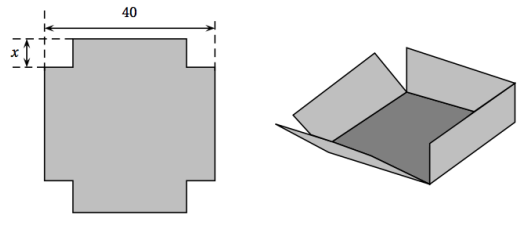
\includegraphics[scale=0.7]{graphics/dm05_patron}
\end{center}

On note $f$ la fonction qui au nombre $x$ associe le volume $f(x)$ en cm$^3$ de la boîte obtenue.

\begin{enumerate}
	\item
	\begin{enumerate}
		\item Déterminer l'ensemble de définition (autrement dit l'ensemble des valeurs de $x$ pour lesquelles le volume $f(x)$ existe), noté $I$, de la fonction $f$.
		\item Calculer $f(5)$ et interpréter le sens concret de ce résultat.
	\end{enumerate}
	\item Déterminer l'expression de $f(x)$ en fonction de $x$ pour $x \in I$.
	\item À l'aide de la trame de graphique suivant pour lequel les unités sont à préciser, tracer la courbe représentative de la fonction $f$ pour $x \in I$.
		\begin{center}
			\tunits{0.75}{0.0015}
			\tdefgrille{0}{21}{1}{1}{0}{5000}{500}{500}
			\tikzset{pointilles/.style={densely dashed,line width=1.5pt}}
			\begin{tikzpicture}[x=\xunit cm,y=\yunit cm]
				%AXES/GRILLE
				\tgrillep[line width=0.4pt,orange!50]
				\draw[line width=0.4pt,orange!50] (0,5000) -- (21,5000) ;
				\axestikz \axextikz*{0,1,...,20} \axeytikz*{0,500,...,4500}
			\end{tikzpicture}
		\end{center}
	\item On répondra aux questions suivantes à l’aide de la représentation graphique de $f$ avec la précision permise par ce graphique.
	
	\textit{On laissera apparents sur le graphique les pointillés utiles pour la lecture graphique.}
	\begin{enumerate}
		\item Donner les éventuels antécédents de 2\,500 par $f$ et interpréter le résultat.
		\item Pour quelles valeurs de $x$ le volume de la boîte est-il inférieur à 2\,000 cm$^3$ ?
		\item Quel volume maximum peut-on obtenir en fabriquant une boîte comme ceci ? Pour quelle valeur de $x$ ce volume maximal est-il atteint ?
	\end{enumerate}
	\item
	\begin{enumerate}
		\item Déterminer graphiquement les solutions de $f(x)=\num{3000}$.
		\item Déterminer, par tabulations successives, une valeur approchée à $10^{-2}$ près de(s) solution(s) de l'équation $f(x)=\num{3000}$.
	\end{enumerate} 
\end{enumerate}

\end{document}